\section{Results}
Presentation of graphs, vary p from 1 to 36
and $n= 2^{14}$

\begin{figure}[h!]
  \centering
  \begin{subfigure}[b]{0.48\textwidth}
    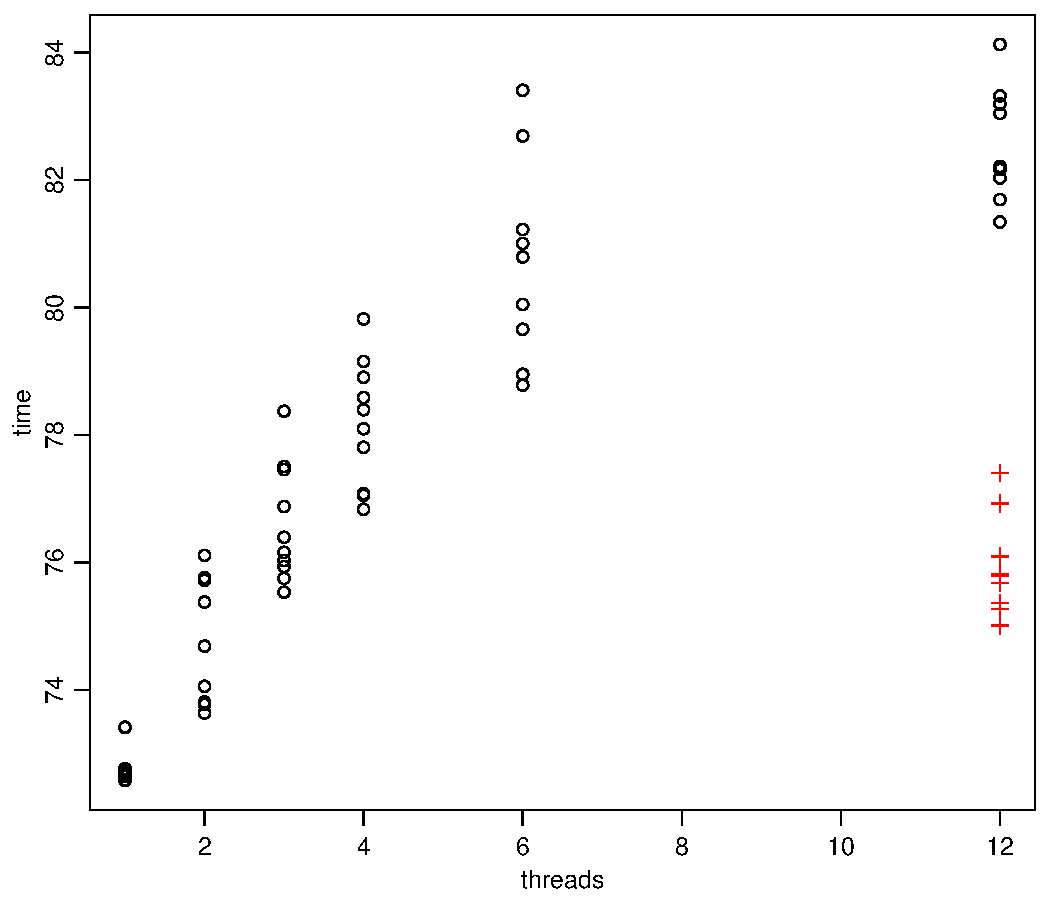
\includegraphics[width=\textwidth]{./Figures/taskc1.pdf}
  \end{subfigure}%
  \quad
  \begin{subfigure}[b]{0.48\textwidth}
    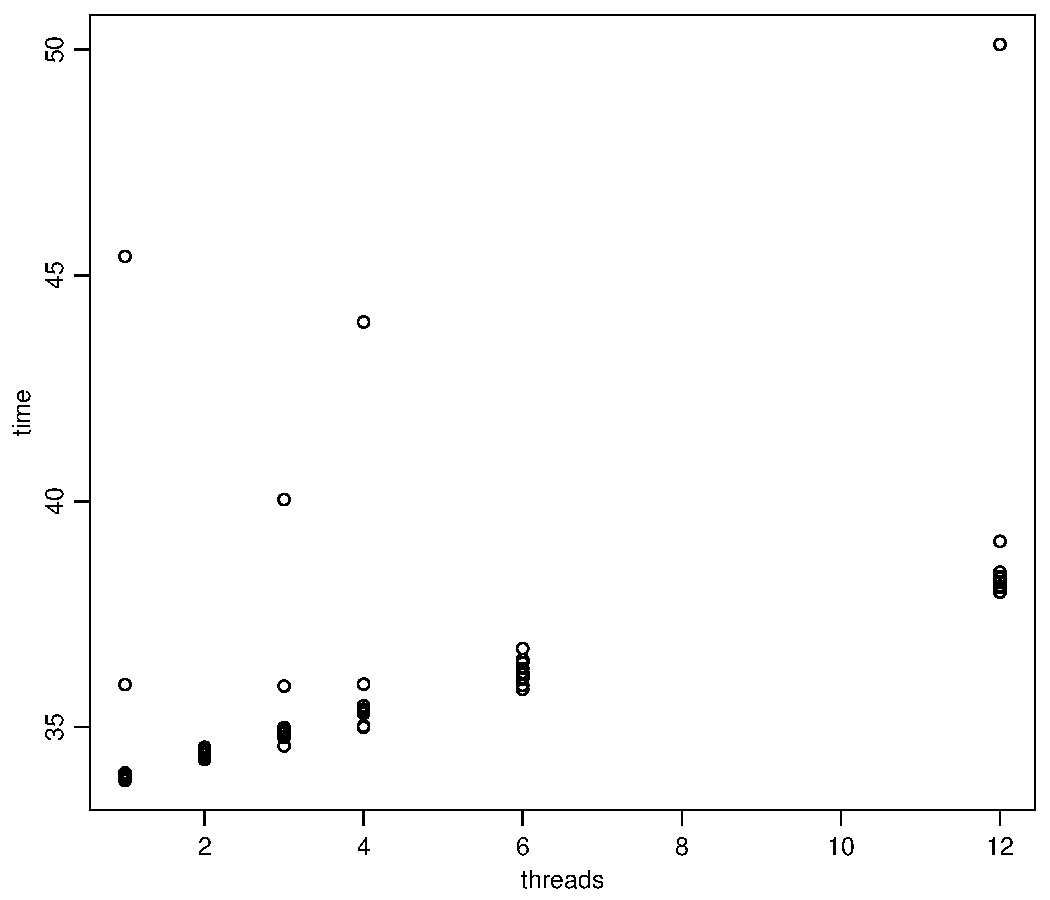
\includegraphics[width=\textwidth]{./Figures/taskc2.pdf}
  \end{subfigure}
          %(or a blank line to force the subfigure onto a new line)
  \vspace{1\baselineskip}
  \caption{Times (in seconds) for running MPI processes vs threads with $n = 2^{14}$. The total number of processors used are 12 per node, so the number of processes per node is 12 - threads. The left figure is run on one node, while the right is run on three nodes. The red crosses are run without any MPI sending at all.}
  \label{fig:taskc}
\end{figure}
%
\begin{figure}[h!]
  \centering
  \begin{subfigure}[b]{0.48\textwidth}
    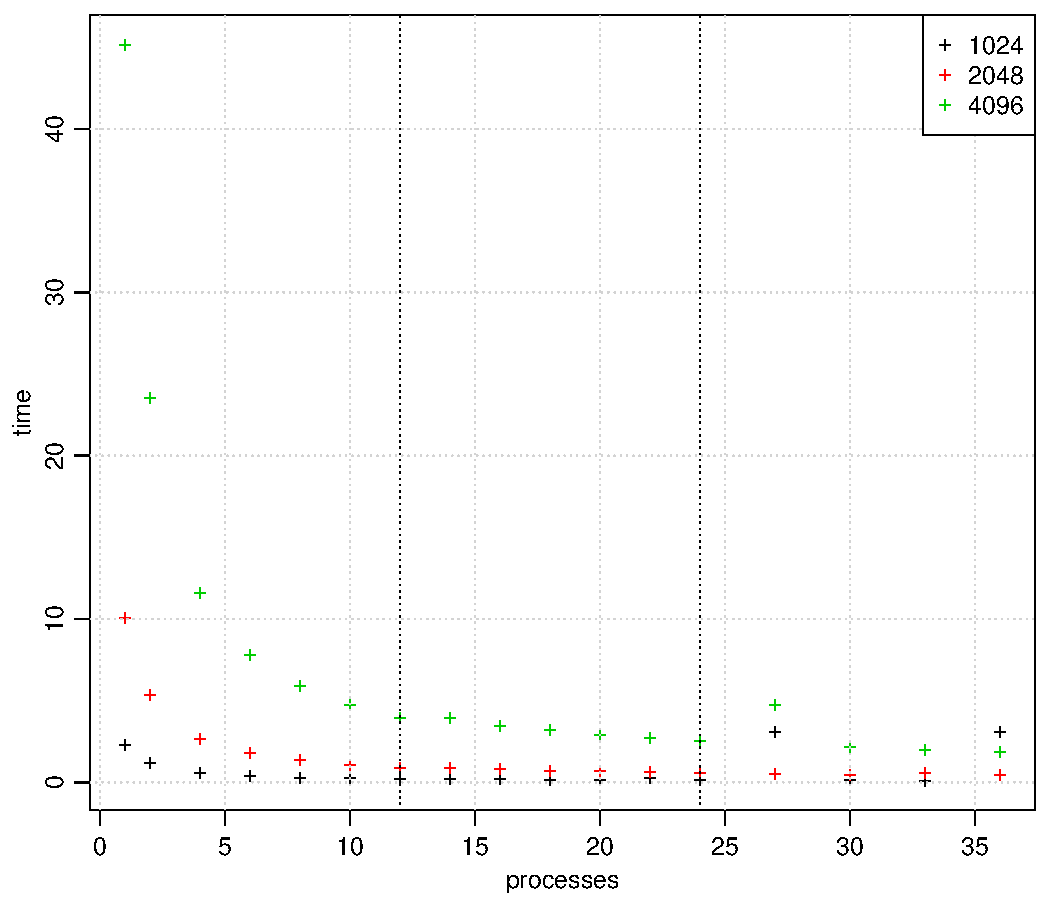
\includegraphics[width=\textwidth]{./Figures/taskbTimeProc1.pdf}
  \end{subfigure}%
  \quad
  \begin{subfigure}[b]{0.48\textwidth}
    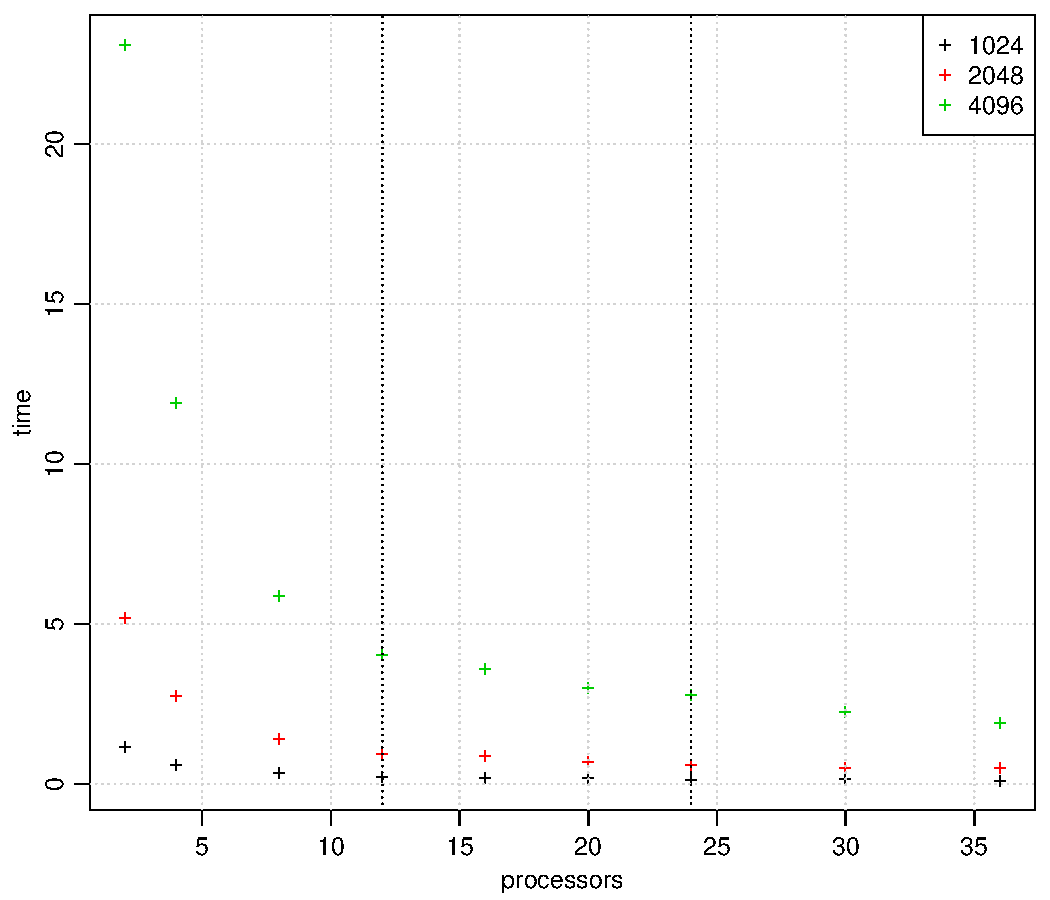
\includegraphics[width=\textwidth]{./Figures/taskbTimeProc2.pdf}
  \end{subfigure}
  \quad
  \begin{subfigure}[b]{0.48\textwidth}
    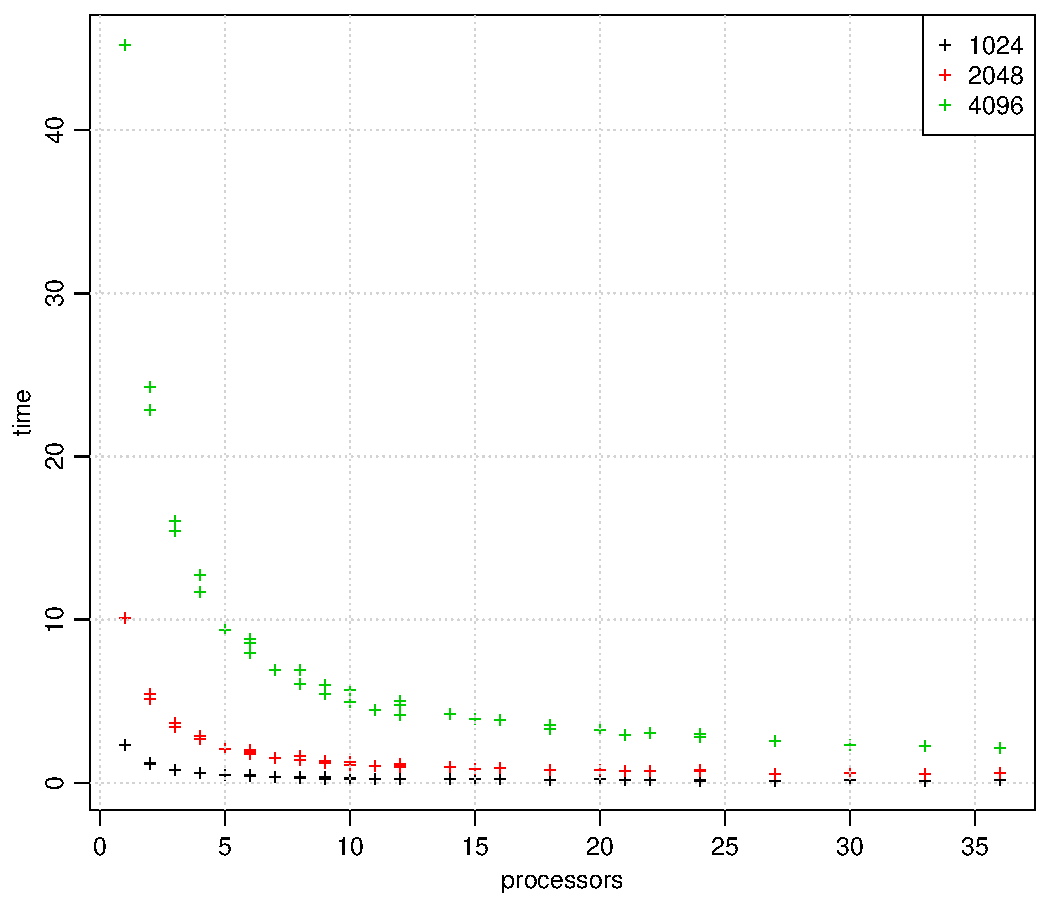
\includegraphics[width=\textwidth]{./Figures/taskbTimeNodesTimesThreads.pdf}
  \end{subfigure}
          %(or a blank line to force the subfigure onto a new line)
  \vspace{1\baselineskip}
  \caption{Times for running problem with different amount of processes. In the upper left figure each process has one thread, while in the upper right, each process has two treads. The problem is run on as few nodes as possible, and the processes are identically distributed among the nodes. The problem size $n$ is specified in the plots. In the bottom figure only one MPI process is run per node. Between 1 and 12 threads are run on each node.}
  \label{fig:time}
\end{figure}
%
\begin{figure}[h!]
  \centering
  \begin{subfigure}[b]{0.48\textwidth}
    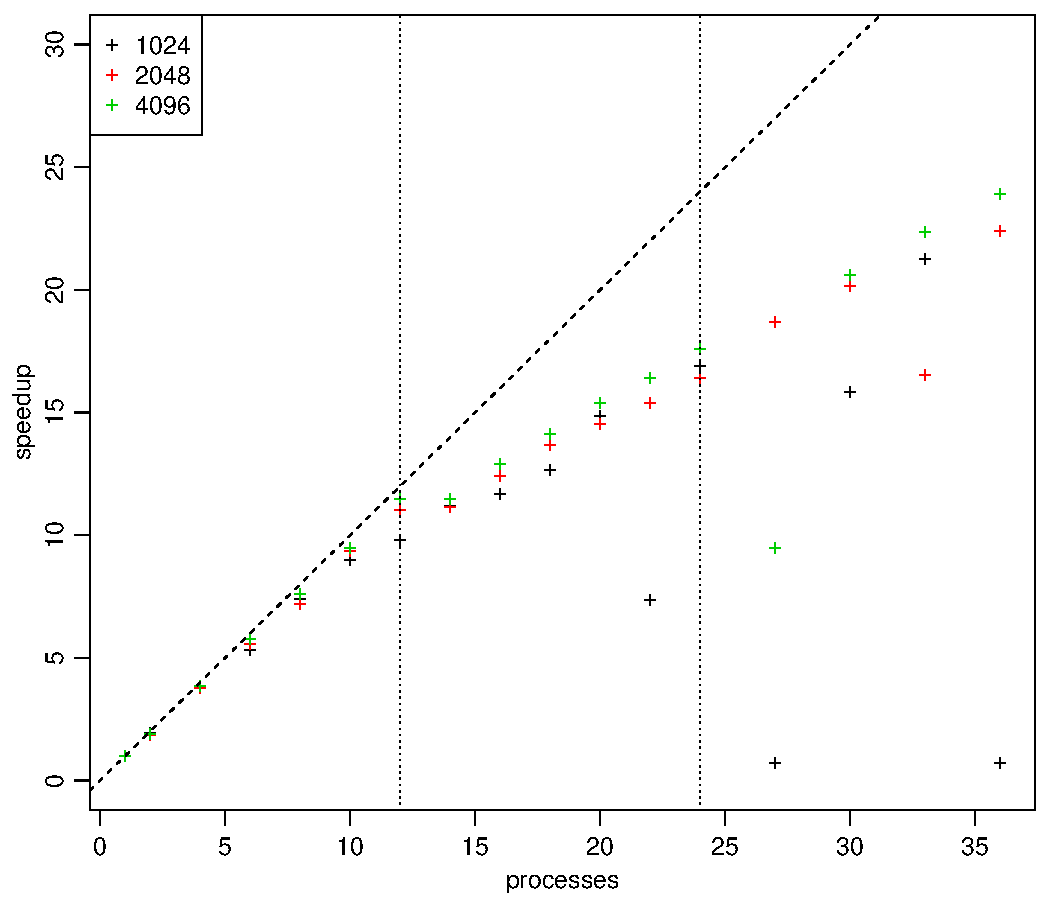
\includegraphics[width=\textwidth]{./Figures/taskbSpeedupProc1.pdf}
  \end{subfigure}%
  \quad
  \begin{subfigure}[b]{0.48\textwidth}
    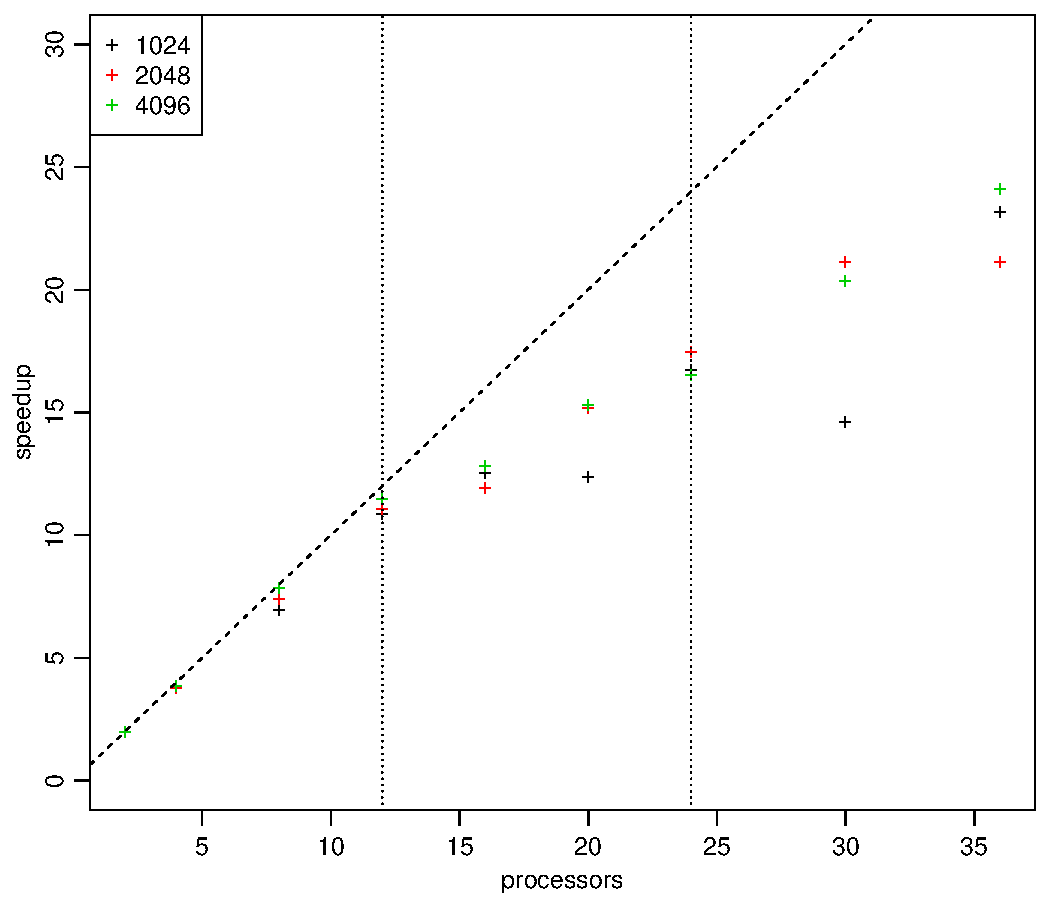
\includegraphics[width=\textwidth]{./Figures/taskbSpeedupProc2.pdf}
  \end{subfigure}
  \quad
  \begin{subfigure}[b]{0.48\textwidth}
    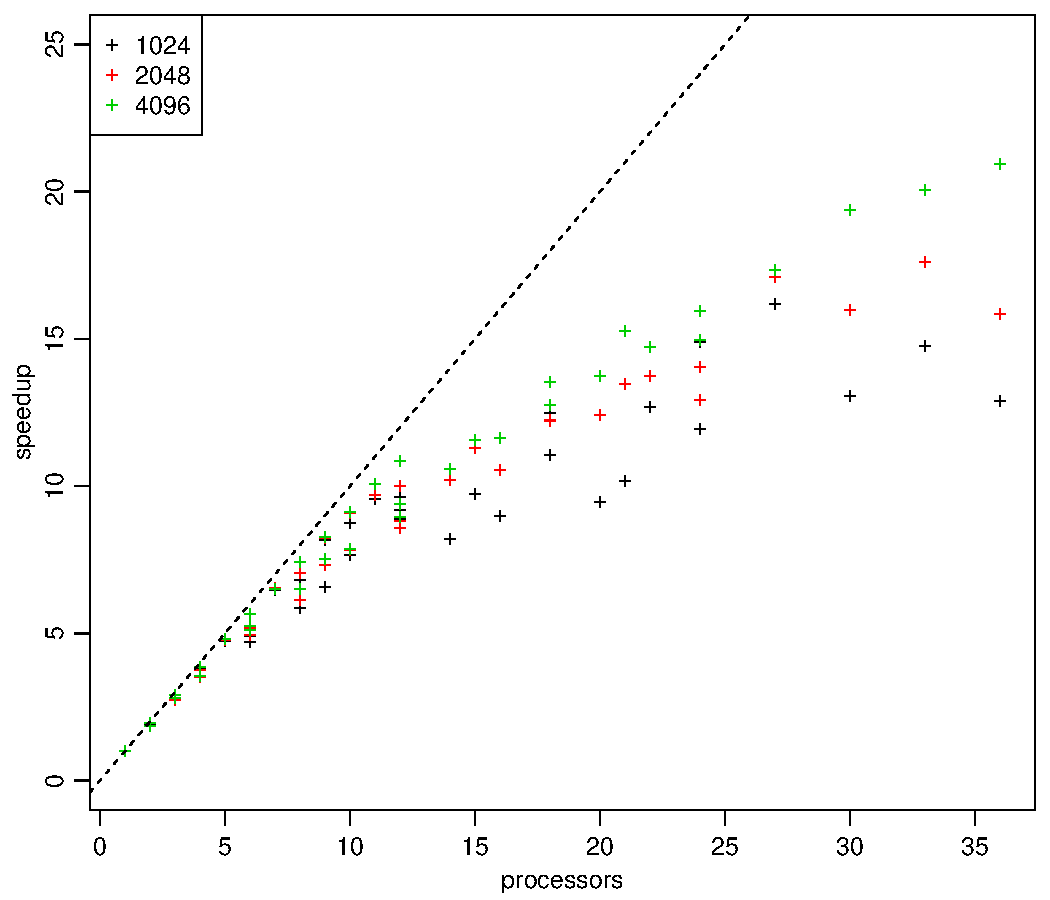
\includegraphics[width=\textwidth]{./Figures/taskbSpeedupNodesTimesThreads.pdf}
  \end{subfigure}
          %(or a blank line to force the subfigure onto a new line)
  \vspace{1\baselineskip}
  \caption{Speedup for running problem with different amount of processes. In the upper left figure each process has one thread, while in the upper right, each process has two treads. The problem is run on as few nodes as possible, and the processes are identically distributed among the nodes. There are drawn vertical lines to show when a new node is utilized, and a line with slope 1. The problem size $n$ is specified in the plots. In the bottom figure only one MPI process is run per node. Between 1 and 12 threads are run on each node.}
  \label{fig:Speedup}
\end{figure}
%
\begin{figure}[h!]
  \centering
  \begin{subfigure}[b]{0.48\textwidth}
    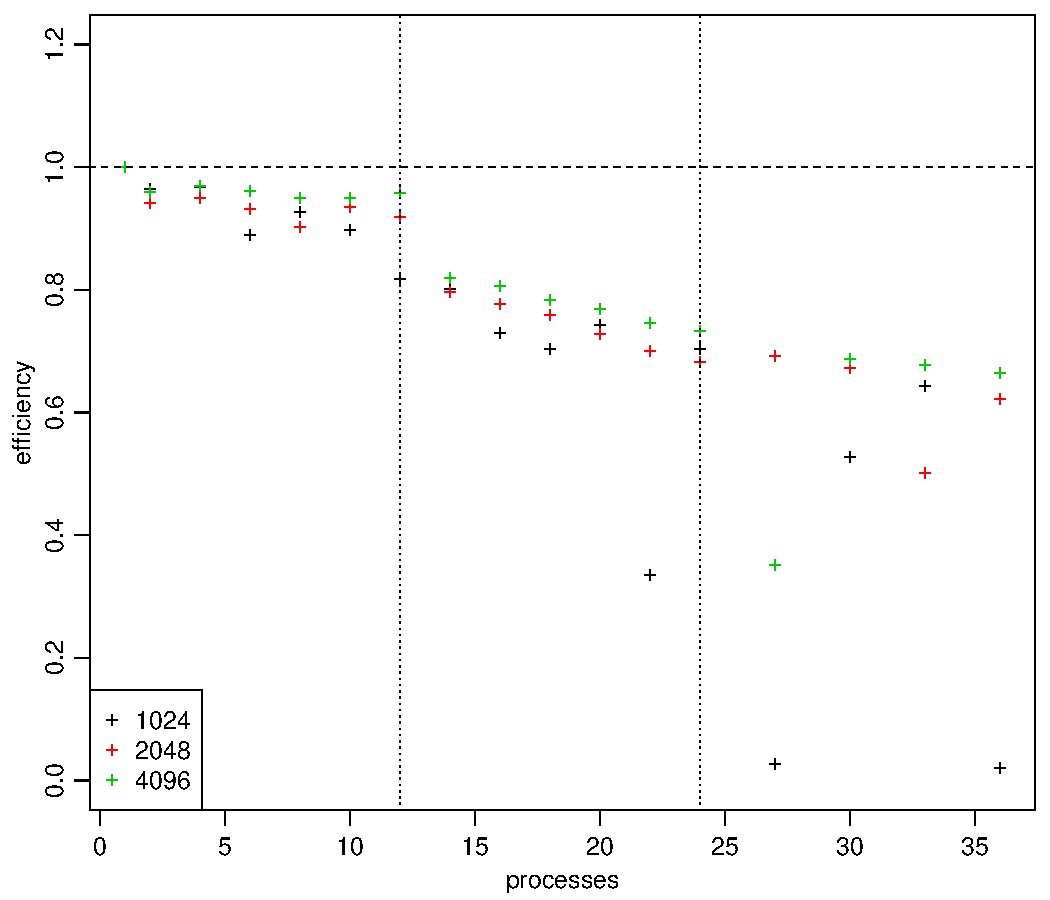
\includegraphics[width=\textwidth]{./Figures/taskbEfficiencyProc1.pdf}
  \end{subfigure}%
  \quad
  \begin{subfigure}[b]{0.48\textwidth}
    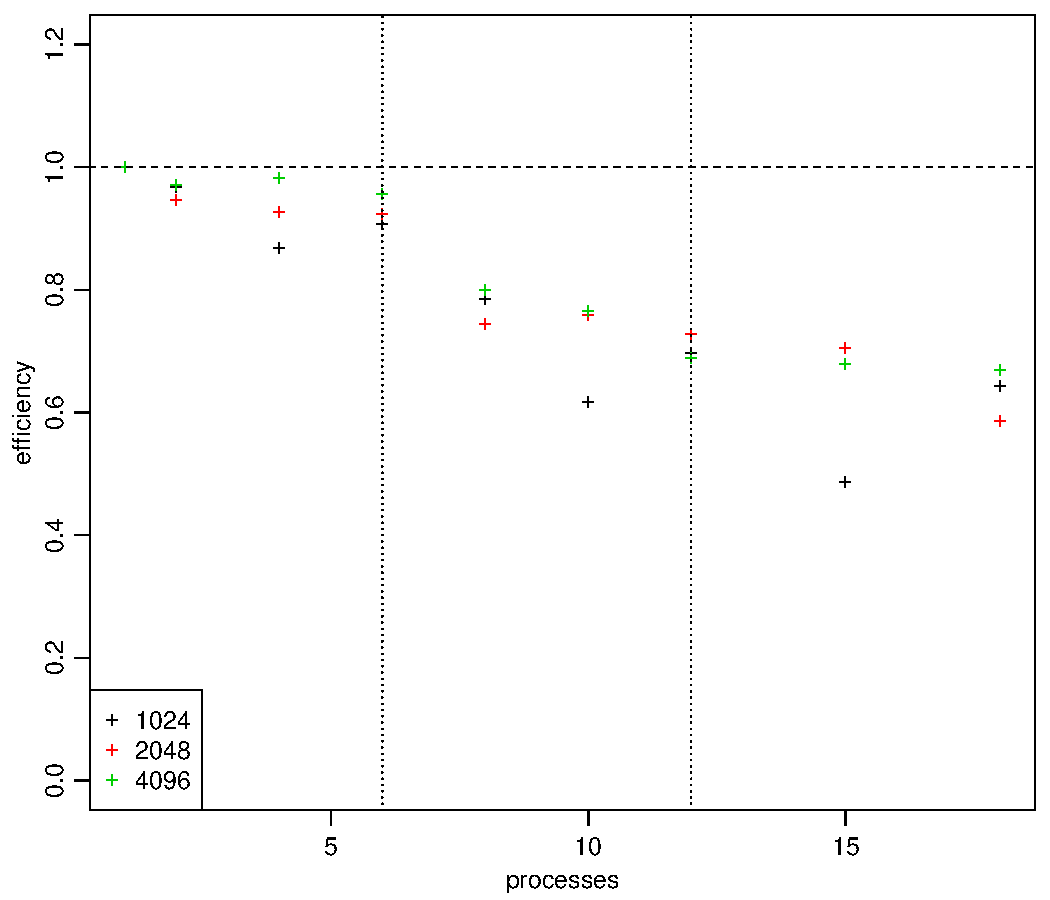
\includegraphics[width=\textwidth]{./Figures/taskbEfficiencyProc2.pdf}
  \end{subfigure}
          %(or a blank line to force the subfigure onto a new line)
  \vspace{1\baselineskip}
  \caption{Efficiency for running problem with different amount of processes. In the upper left figure each process has one thread, while in the upper right, each process has two treads. The problem is run on as few nodes as possible, and the processes are identically distributed among the nodes. There are drawn vertical lines to show when a new node is utilized, and a horizontal line at 1. The problem size $n$ is specified in the plots. In the bottom figure only one MPI process is run per node. Between 1 and 12 threads are run on each node.}
  \label{fig:Efficiency}
\end{figure}
%
\begin{figure}[h!]
  \centering
  \begin{subfigure}[b]{0.48\textwidth}
    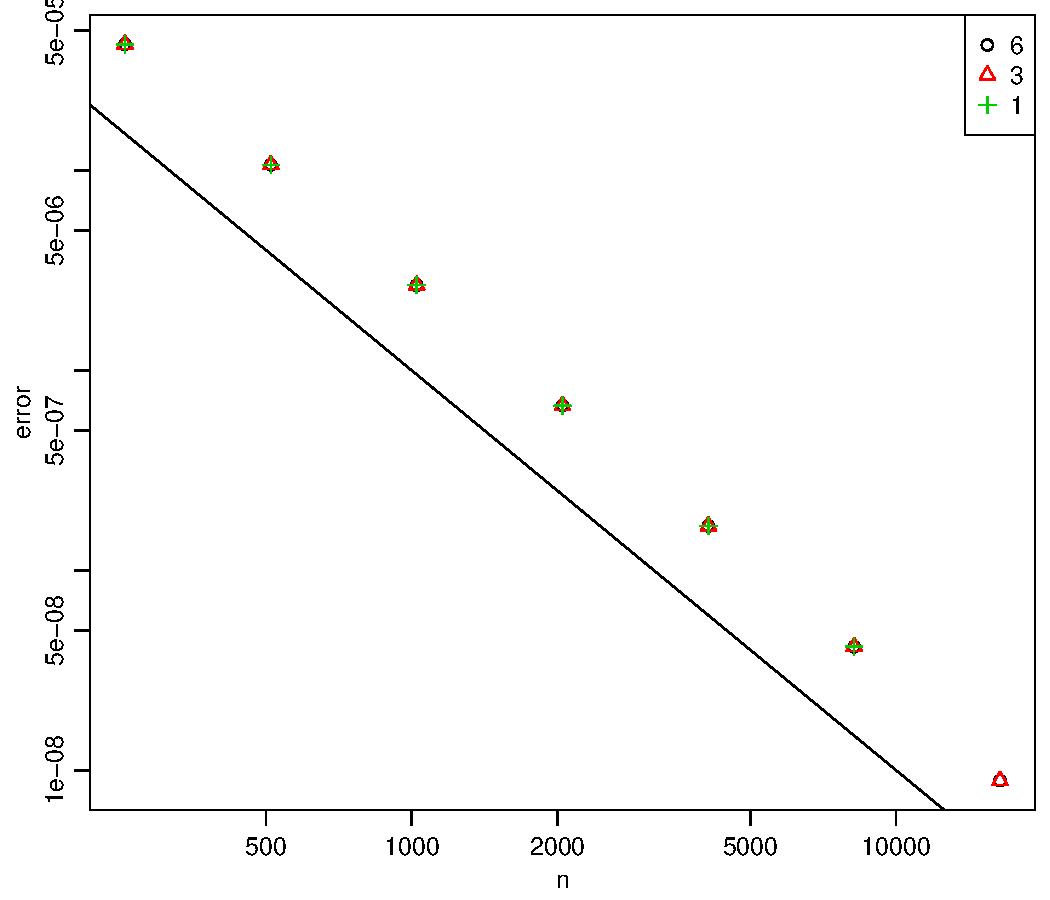
\includegraphics[width=\textwidth]{./Figures/errVsn.pdf}
  \end{subfigure}%
  \quad
  \begin{subfigure}[b]{0.48\textwidth}
    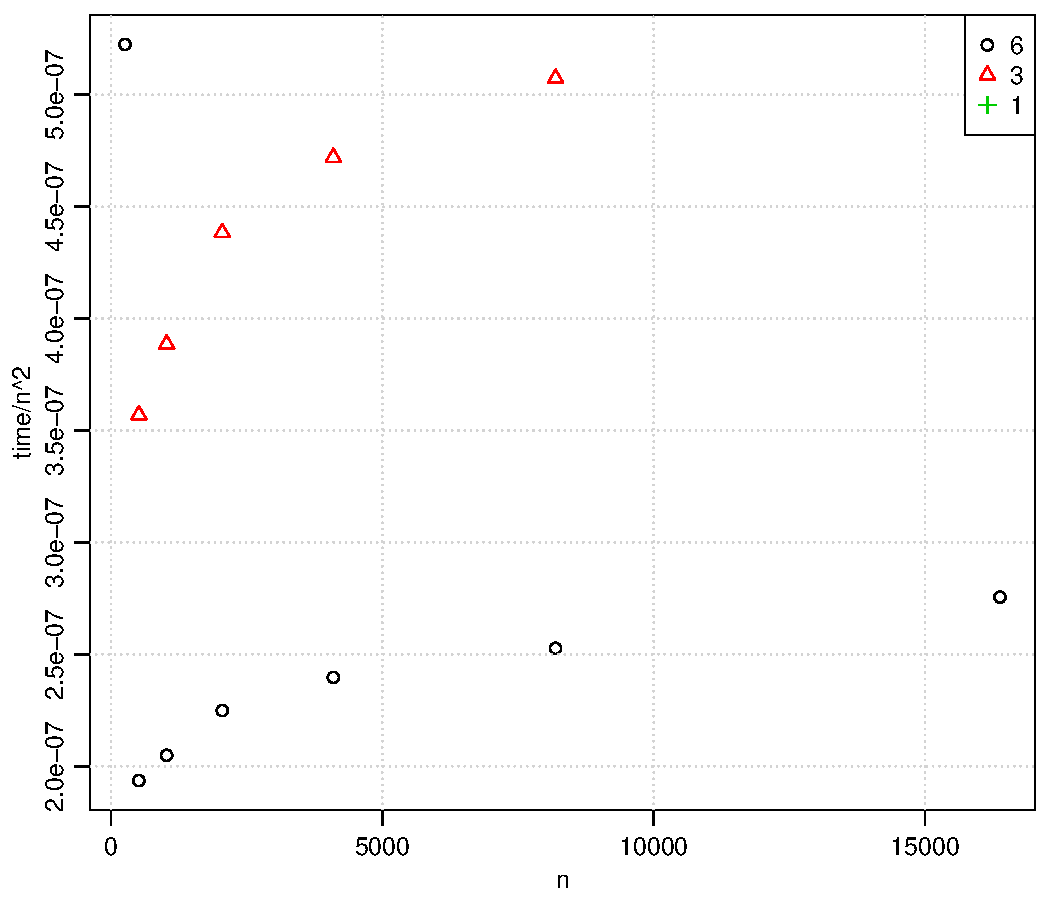
\includegraphics[width=\textwidth]{./Figures/timeOverN2Vsn.pdf}
  \end{subfigure}
          %(or a blank line to force the subfigure onto a new line)
  \vspace{1\baselineskip}
  \caption{The left figure shows a loglog plot of the error as function of $n$. A reference line with slope $-2$ is drawn. The problem is run on two threads, with the number of processes specified in the legend. Only one node is used. The right figure hows $time/n^2$.}
  \label{fig:conv}
\end{figure}



